\documentclass[conference]{IEEEtran}
\IEEEoverridecommandlockouts
\usepackage{cite}
\usepackage{amsmath,amssymb,amsfonts}
\interdisplaylinepenalty=2500
\usepackage{graphicx}
\usepackage{xcolor}
\usepackage{colortbl}  % light shading of the FADO rows of Table III
\usepackage{booktabs}
\usepackage{multirow}
\usepackage{array}
\newcolumntype{L}[1]{>{\raggedright\arraybackslash}p{#1}}
% IEEE allows only figures and tables as floats (IEEEtran_HOWTO, Sec. X-B):
% the pseudocode is set with algpseudocode inside a figure.
\usepackage{algpseudocode}
\usepackage{url}

\newtheorem{proposition}{Proposition}
\newtheorem{remark}{Remark}
\newcommand{\TODO}[1]{\textcolor{red}{\textbf{[TODO: #1]}}}
\newcommand{\tbd}{\textcolor{red}{\textbf{TBD}}}
\newcommand{\fado}{\textsc{FADO}}
\newcommand{\ara}{\textsc{Aranyani}}
\newcommand{\arf}{\textsc{ARF}}
\newcommand{\rfr}{\textsc{RFR}}
\newcommand{\adult}{\textsc{Adult}}
\newcommand{\folk}{\textsc{Folktables}}
\newcommand{\sig}[1]{^{\scriptscriptstyle #1}}
\newcommand{\tnote}[1]{\vspace{2pt}\parbox{\linewidth}{\footnotesize #1}}
% new row of authors in the IEEEtran author block
\makeatletter\newcommand{\linebreakand}{\end{@IEEEauthorhalign}\hfill\mbox{}\par\mbox{}\hfill\begin{@IEEEauthorhalign}}\makeatother

\begin{document}

% Template rules: no abbreviations, subtitles, math, or symbols in the title.
\title{Adaptive Fairness Constraints for Online Learning\\Under Concept Drift}
\author{\IEEEauthorblockN{Tiago Silva}
\IEEEauthorblockA{\textit{CISUC, Dept. of Informatics Engineering} \\
\textit{University of Coimbra}\\
Coimbra, Portugal \\
tds@student.uc.pt}
\and
\IEEEauthorblockN{Bruno Veloso}
\IEEEauthorblockA{\textit{INESC TEC, Faculty of Economics} \\
\textit{University of Porto}\\
Porto, Portugal \\
bruno.m.veloso@inesctec.pt}
\and
\IEEEauthorblockN{Jo\~{a}o Gama}
\IEEEauthorblockA{\textit{INESC TEC, Faculty of Economics} \\
\textit{University of Porto}\\
Porto, Portugal \\
joao.gama@inesctec.pt}
\linebreakand
\IEEEauthorblockN{Pedro Henriques Abreu}
\IEEEauthorblockA{\textit{CISUC, Dept. of Informatics Engineering} \\
\textit{University of Coimbra}\\
Coimbra, Portugal \\
pha@dei.uc.pt}
}

\maketitle

% Template rules: no math, symbols, special characters, footnotes, or
% citations in the abstract. Every number below is derived in
% supplementary/paper_numbers.md or printed in Table III.
\begin{abstract}
Online learning systems in nonstationary environments must remain both predictive and fair as the data distribution evolves.
Existing fairness-aware learners optimize a fixed regularizer, ignoring concept drift, while drift-adaptive streaming methods enforce no
fairness. In this context, we propose Fairness-Aware Drift-Aware Online Learning (FADO), an online learner that enforces fairness through an adaptive
constraint and responds to drift through a reaction controller. Instead of weighting the fairness penalty by a constant chosen in advance,
FADO bounds demographic parity and treats the penalty weight as the Lagrange multiplier of that bound, updated online from a per-sample
estimate of each group's disparity that we prove to be unbiased. A drift detector and a fairness monitor reset the penalty's statistics
when the stream changes, and the controller temporarily raises the learning rate after a detected drift. Over 30 seeds, on a natural
cross-year shift in census income data and on four types of concept drift injected into a second income stream, FADO lowers demographic
parity by 25 to 33 percent relative to the same forest with a fixed weight, and is significantly fairer than all three published
baselines over the whole stream and after the drift. After an abrupt feature drift, it even
outperforms, on every metric, a fixed-weight forest that was tuned on the test data, which a real
deployment cannot do.
\end{abstract}
\begin{IEEEkeywords}
fairness-aware online learning, concept drift, constrained learning, drift detection, group fairness, oblique decision forests
\end{IEEEkeywords}

% =====================================================================
\section{Introduction}
\label{sec:intro}
The growing adoption of machine learning (ML) systems in critical decision-making domains, including healthcare~\cite{8474918}, criminal
justice~\cite{10467221}, and hiring~\cite{10.1145/3351095.3372828}, where their predictions may directly affect individuals and society, makes optimizing for
performance an insufficient objective; models must also satisfy fairness requirements to ensure equitable treatment across individuals or groups of
individuals~\cite{10.1145/3457607}. In this regard, among the fairness literature, \emph{group fairness}~\cite{10.1145/2090236.2090255} has emerged as one of the most
widely studied paradigms, aiming to ensure that predictive behavior is balanced across populations defined by sensitive attributes such as gender, race, or age.
Common formulations include demographic parity (DP), equal opportunity, and equalized odds (EO), each imposing statistical constraints on model outcomes across
groups (sometimes mutually incompatible)~\cite{10.1145/2090236.2090255,NIPS2016_6a9659fe}. Most existing fairness-aware models are, unfortunately, developed under the
assumption of a stationary data distribution. In practice, real-world environments are inherently dynamic, and properties of data evolve over
time due to policy changes, behavioral shifts, seasonal effects, economic fluctuations, or other social transformations. This phenomenon, commonly referred to as
concept drift, occurs when the relationship between input variables and target outcomes changes over time, causing previously learned decision boundaries to
become outdated. Different forms of concept drift~\cite{DBLP:journals/corr/WebbHCNP15} require different adaptation strategies and can degrade performance when
models fail to adjust. Drift also threatens fairness: shifting distributions alter the statistical relationships that support fairness guarantees, increasing bias
against some groups. To address this challenge, the online learning and data stream mining literature has proposed numerous adaptive methods capable of detecting
and responding to concept drift in real time. These approaches often rely on drift detection mechanisms combined with incremental learning strategies to maintain
predictive accuracy under nonstationary conditions. However, the majority of existing methods focus primarily on predictive
utility~\cite{10.1007/s10994-017-5642-8,KLAIBER20231261}, while fairness considerations remain comparatively underexplored. As a result, fairness guarantees
established during training may deteriorate over time even when predictive accuracy remains relatively stable~\cite{deho2024faircomparativeevaluationfairness}. This limitation is particularly
critical in high-stakes applications, where persistent fairness violations may remain undetected for extended periods, compromising trustworthiness, reinforcing
societal inequalities, and causing objective harm to affected groups. These observations highlight an important gap in the literature and motivate the following
research questions (RQs):
\begin{itemize}
\item \textbf{RQ1:} To what extent does concept drift affect group fairness metrics in online learning settings?
\item \textbf{RQ2:} Can adaptive drift detection and response mechanisms preserve fairness guarantees while maintaining predictive performance over time?
\end{itemize}

Based on these research questions, this work investigates fairness-aware online learning under concept drift. We introduce \textbf{F}airness-\textbf{A}ware \textbf{D}rift-Aware \textbf{O}nline
Learning (\fado{}), a framework built on three mechanisms: an \emph{adaptive fairness constraint}, which states fairness as a bound on the fairness metric and
learns the weight of the fairness penalty online as the Lagrange multiplier of that bound, instead of fixing it in advance; a dual-threshold drift detector,
complemented by a fairness monitor, whose confirmed drifts reset the fairness penalty's running statistics; and a reaction controller that modulates the optimizer
learning rate and a routing temperature in response to detected change. \fado{} applies these mechanisms to a soft-routed fair oblique decision forest. Our
central hypothesis is that fairness degradation under concept drift can be mitigated by enforcing fairness as a constraint whose price adapts to the data, coupled
with explicit drift detection and response, allowing the model to maintain both predictive utility and equitable treatment across groups in
nonstationary environments.

To evaluate this hypothesis, we run our evaluation on two complementary testbeds. \folk{} (American Community Survey (ACS) Income,
California) contributes a natural cross-year shift between 2015 (training) and 2017--2018 (prequential test), and \adult{} serves as a controlled testbed into
whose stream we inject four types of concept drift~\cite{10.1145/3770855.3819070}, one per scenario. \fado{} is compared against three streaming baselines
spanning the accuracy/fairness/adaptivity design space: the Adaptive Random Forest (\arf{})~\cite{10.1007/s10994-017-5642-8}, an accuracy-oriented ensemble with
drift detection but no fairness mechanism; robust fairness regularization (\rfr{})~\cite{jiang2023chasingfairnessdistributionshift}, a sharpness-aware
fairness-reweighted method without adaptive drift handling; and \ara{}~\cite{chowdhury2024enhancing}, which shares \fado{}'s forest model but uses a fixed
fairness weight and no drift handling, and therefore isolates \fado{}'s contribution. To separate the benefit of adapting the weight from that of a larger one, we
also give this baseline, in hindsight, the constant weight that \fado{} reaches online. The main contributions of this work are:
\begin{itemize}
\item \fado{}, a fairness-aware online learning framework that combines an adaptive fairness constraint, a dual-threshold ADWIN drift detector with a
fairness monitor, and a reaction controller acting on the learning rate and on a routing temperature that \fado{} introduces;
\item A formulation that keeps a bound on the demographic parity
of the predictions and treats the penalty weight as its dual price, tracked online, together with a per-sample Horvitz--Thompson estimate of each group's disparity that we prove unbiased and that drives both the price and the fairness monitor;
\item An empirical analysis over 30 seeds, on a natural cross-year shift on \folk{} and on four injected drift types on \adult{}, of how concept drift affects group
fairness over the stream, comparing \fado{} against the \arf{}, \rfr{}, and controller-free \ara{} baselines, and against \ara{} given \fado{}'s weight in
hindsight, with paired, multiplicity-corrected tests, together with an analysis of how often and how fast \fado{} detects each drift; code, per-seed results,
and the scripts that generate every table and number are released.
\end{itemize}

The remainder of this paper is organized as follows. Section~\ref{sec:related} reviews related work and identifies the limitations that motivate \fado{}.
Section~\ref{sec:problem} formalizes the online setting, the fairness metrics, and the constrained problem. Section~\ref{sec:method} presents \fado{} and the
experimental design. Section~\ref{sec:results} reports and discusses the results in light of the two research questions, and Section~\ref{sec:conclusion}
concludes and outlines future work.

% =====================================================================
\section{Related Work}
\label{sec:related}
Following a widely used taxonomy in the fair machine learning literature~\cite{Salazar_2026}, we group related work into three categories: (i) pre-processing,
(ii) in-processing, and (iii) post-processing methods, and then summarize the limitations that motivate this work.

\subsection{Pre-Processing Methods}
Pre-processing methods aim to mitigate bias in the data before the training stage of a model. Xiong et
al.~\cite{Xiong_Dalmasso_Mishler_Potluru_Balch_Veloso_2024} propose leveraging training samples reweighting to satisfy demographic parity while minimizing
distributional distortion using the Wasserstein distance to the original dataset. Although effective, this method does not account for concept drift, nor does it
prove robustness to other forms of fairness violations, which limits its applicability in dynamic environments. Zeng et
al.~\cite{zeng2024fairrrpreprocessinggroupfairness} propose a different approach that contrasts with the aforementioned, modifying the actual data labels by treating
the removal of discrimination from the training dataset as a randomized response problem. The main contribution of this work is the provision of a theoretical
bridge between pre-processing techniques and downstream Bayes-optimal classifiers, and the fact that it is model agnostic: because it only alters the training
labels, users do not need to modify their current pipelines. However, this method also does not account for concept drift or its impact, and it is limited by
the binary setup, meaning it only works with binary sensitive attributes and binary outcomes.

\subsection{In-Processing Methods}
In-processing methods incorporate fairness constraints directly into the learning algorithm. Four lines are especially relevant to our work.

Chowdhury et al.~\cite{chowdhury2024enhancing} propose \ara{}, an online fair-learning ensemble of soft-routed oblique decision trees in which the
demographic-parity penalty is enforced at the level of individual routing nodes, inducing a parameter-isolation property that keeps the per-step fairness gradient
cheap and lets the ensemble track running per-group statistics rather than storing past samples. \ara{} starts from node-level fairness constraints but relaxes
them into a regularizer whose weight is a fixed hyperparameter, and it has no mechanism for drift. \fado{} uses the same forest model and addresses
both limitations.

Gomes et al.~\cite{10.1007/s10994-017-5642-8} propose \arf{}, a streaming ensemble of Hoeffding trees with per-tree warning and drift detectors that swap in
background trees on confirmed drift. \arf{} is the standard streaming-adaptation baseline but is purely accuracy-oriented; we treat it as a representative
adaptive-but-not-fair baseline.

Jiang et al.~\cite{jiang2023chasingfairnessdistributionshift} model distribution shift as a bounded weight-space perturbation and optimize for worst-case
fairness under that perturbation, producing the sharpness-aware reweighting (\rfr{}) that we use as our fair-but-not-adaptive baseline.

Finally, fairness can be imposed as a constraint rather than as a weighted penalty. Zafar et al.~\cite{zafar2017fairnessconstraintsmechanismsfair} bound a covariance proxy of disparate
impact, Agarwal et al.~\cite{agarwal2018reductionsapproachfairclassification} reduce fair classification to a saddle-point problem solved by a sequence of cost-sensitive learners, and Cotter
et al.~\cite{cotter2018optimizationnondifferentiableconstraintsapplications} optimize nondifferentiable rate constraints with a proxy-Lagrangian game. These methods solve the problem offline on a fixed
training set; online convex optimization with long-term constraints~\cite{mahdavi2012trading} provides the primal--dual template that \fado{} follows one sample at a
time.

\subsection{Post-Processing Methods}
Post-processing approaches transform an already-trained classifier's outputs. Hardt et al.~\cite{NIPS2016_6a9659fe} introduce randomized threshold adjustments
that equalize group error rates and remain the standard model-agnostic baseline; Mishler et al.~\cite{Mishler_2021} extend the idea to counterfactual equalized
odds in intervention settings (at the cost of strong causal assumptions); Small et al.~\cite{Small_2024} replace fixed randomization regions with smooth monotonic
probability curves to recover individual fairness. None of these methods touch the training loop, so none of them adapt under drift; we mention them for
completeness rather than as direct comparators.

\subsection{Main Limitations of Prior Work}
\label{sec:related:limitations}
Notwithstanding the significant contributions of the families surveyed above, we identify four main limitations that jointly motivate this work and the design
of \fado{}:
\begin{itemize}
\item \textbf{L1 -- Static fairness assumption.} Once the protected-attribute conditional or the label distribution shifts, the fairness guarantees obtained at
training time provide no protection at deployment;
\item \textbf{L2 -- Adaptive methods are accuracy-oriented.} Streaming ensembles such as \arf{}~\cite{10.1007/s10994-017-5642-8} explicitly detect and react to drift
but do so purely on the predictive-error signal, with no mechanism for tracking or correcting fairness violations;
\item \textbf{L3 -- Existing fair online learners do not react to drift.} \ara{}~\cite{chowdhury2024enhancing} provides memory-efficient online fairness, but its
regularizer is nonadaptive: when the distribution moves it continues to optimize the same penalty with the same fixed weight, although the weight that keeps
disparity acceptable changes with the data, and convergence to the new optimum is slow;
\item \textbf{L4 -- Drift-aware fair methods rely on assumptions that do not transfer to streams.} Approaches such
as~\cite{jiang2023chasingfairnessdistributionshift} treat distribution shift as a bounded weight-space perturbation, which is useful in worst-case analysis but
does not yield an actionable online detector or controller, and constrained fair learners~\cite{zafar2017fairnessconstraintsmechanismsfair,cotter2018optimizationnondifferentiableconstraintsapplications,agarwal2018reductionsapproachfairclassification}
solve their problem offline.
\end{itemize}
\fado{} addresses L1--L4 directly with (i)~an
adaptive fairness constraint, whose dual price replaces the fixed fairness weight; (ii)~an ADWIN-based dual-threshold detector on the online error stream and a
fairness monitor on a per-sample disparity signal, whose confirmed drifts reset the regularizer's running statistics; and (iii)~a reaction controller that
modulates the optimizer learning rate and a routing temperature added to the forest on warning and confirmation events.

% =====================================================================
\section{Problem Statement}
\label{sec:problem}
This section formalizes the online learning setting, the group fairness metrics, and the 
constrained optimization problem that \fado{} solves.

\subsection{Online Learning Setting}
\label{sec:problem:online}
We consider an online binary classification problem over a data stream $\{(x_t, y_t, a_t)\}_{t=1}^{T}$, where $x_t \in \mathbb{R}^d$ is the feature vector
observed at time $t$, $y_t \in \{0,1\}$ is the binary target label, and $a_t \in \mathcal{A}$ is a sensitive attribute taking values in a finite set with
$|\mathcal{A}|=K \ge 2$. Following the formulation of previous work~\cite{chowdhury2024enhancing,zhang2019fahtadaptivefairnessawaredecision}, at each time step the learner receives $x_t$,
produces a prediction $\hat{y}_t = \arg\max f_t(x_t)$, then observes $(y_t, a_t)$ and updates its parameters under a prequential, test-then-train protocol. The
fairness formulation introduced below supports arbitrary $K$; in our study each dataset has one binary protected attribute (sex), so $K=2$.

\subsection{Group Fairness Metrics}
\label{sec:problem:metrics}
We focus on \emph{group fairness}, which assesses whether model behavior is statistically similar across protected groups. \ara{}~\cite{chowdhury2024enhancing}
defines demographic parity on the forest's outputs for two groups leaving the implementation to more groups and to equalized odds for future work; we measure
fairness on the \emph{predictions}, in a form that holds for any number of groups. Let $\mathcal{A}_t \subseteq \mathcal{A}$ denote the set of sensitive groups observed
within the current evaluation window, and let $\hat{p}_a = \mathbb{E}[\hat{y} \mid a]$ be the positive-prediction rate for group $a \in \mathcal{A}_t$. We define the
unweighted mean group rate as:
\begin{equation}
\bar{p} = \frac{1}{|\mathcal{A}_t|}\sum_{a' \in \mathcal{A}_t}\hat{p}_{a'},
\end{equation}
i.e., the average positive-prediction rate across the observed groups. The \emph{demographic parity violation} is then the worst-case deviation of any group's
positive-prediction rate from this mean:
\begin{equation}
D_a = \bar{p}-\hat{p}_a, \qquad \mathrm{DP} = \max_{a \in \mathcal{A}_t}\left|D_a\right|,
\label{eq:dp}
\end{equation}
which is bounded between $0$ (perfect parity) and $1$. DP measures bias in the prediction marginal and is sensitive to differences in base rates across groups.
We adopt this mean-from-average form rather than the more common pairwise gap $\max_{a,a'}|\hat p_a - \hat p_{a'}|$ because it mirrors the node-level
regularizer as we implement it (Section~\ref{sec:method:model}). For a binary attribute ($K=2$) this form
reduces to $\mathrm{DP}=\tfrac{1}{2}\,|\hat p_0 - \hat p_1|$, equivalent up to a factor of two to the textbook pairwise gap.

We also report \emph{equalized odds}, the same deviation measured within each true-label class. With $\hat p_{a|y}=\mathbb{E}[\hat y\mid a,y]$ and
$\bar p_y$ its mean across the observed groups:
\begin{equation}
\mathrm{EO} = \max_{y \in \{0,1\}}\ \max_{a \in \mathcal{A}_t}\left|\hat{p}_{a|y} - \bar{p}_y\right|.
\end{equation}
Restricting it to $y{=}1$ gives equal opportunity. EO separates bias from differences in base rates. We report it but do not optimize it: constraining EO in 
\fado{} would also need a label-conditional version of the per-sample signal~\eqref{eq:ht} leaving the implementation to future work. 

\subsection{From a Fixed Penalty to a Fairness Constraint}
\label{sec:problem:constraint}
\ara{}~\cite{chowdhury2024enhancing} states fairness as constraints on the forest's internal routing nodes, but then relaxes them into a regularized objective
$\mathcal{L}_{\mathrm{CE}}+\lambda\,\mathcal{L}_{\text{fair}}$ (Section~\ref{sec:method:model}) whose weight $\lambda$ is fixed in advance, a knob with no
meaning outside the dataset on which it was tuned. What a deployment can state and defend instead is a tolerance: the model's demographic parity must not
exceed $\varepsilon$. We therefore pose:
\begin{equation}
\min_\theta\ \mathbb{E}\big[\mathcal{L}_{\mathrm{CE}}(\theta)\big]\quad\text{s.t.}\quad \mathrm{DP}(\theta)\le\varepsilon,
\label{eq:cons}
\end{equation}
and ask the learner to satisfy it \emph{at every point of a drifting stream}. Under drift the multiplier that makes~\eqref{eq:cons} 
bind changes over time: the weight that keeps disparity acceptable before a shift is too small after a shift that widens the gap between groups, 
and needlessly costly when the stream is already fair, so it must be estimated online rather than tuned once.

% =====================================================================
\section{Methodology and Experimental Design}
\label{sec:method}
\fado{} consists of three mechanisms (Fig.~\ref{fig:drift-pipeline}): (i)~an adaptive fairness
constraint, whose dual price replaces a fixed fairness weight (Section~\ref{sec:method:lambda}); (ii)~drift detection with forgetting, in which a
dual-threshold ADWIN detector on the error stream and a fairness monitor on a per-sample disparity signal reset the fairness statistics on confirmed drift; and
(iii)~a reaction controller on the learning rate and on a routing temperature that \fado{} adds to the forest (both in Section~\ref{sec:method:drift}).
They act on a fair soft oblique forest~\cite{chowdhury2024enhancing}, which we summarize only as far as \fado{} uses it (Section~\ref{sec:method:model}).
Sections~\ref{sec:method:data}--\ref{sec:method:reproducibility} then describe datasets, drift scenarios, baselines, hyperparameter selection, the evaluation
protocol, and reproducibility.
\begin{figure*}[t]
\centering
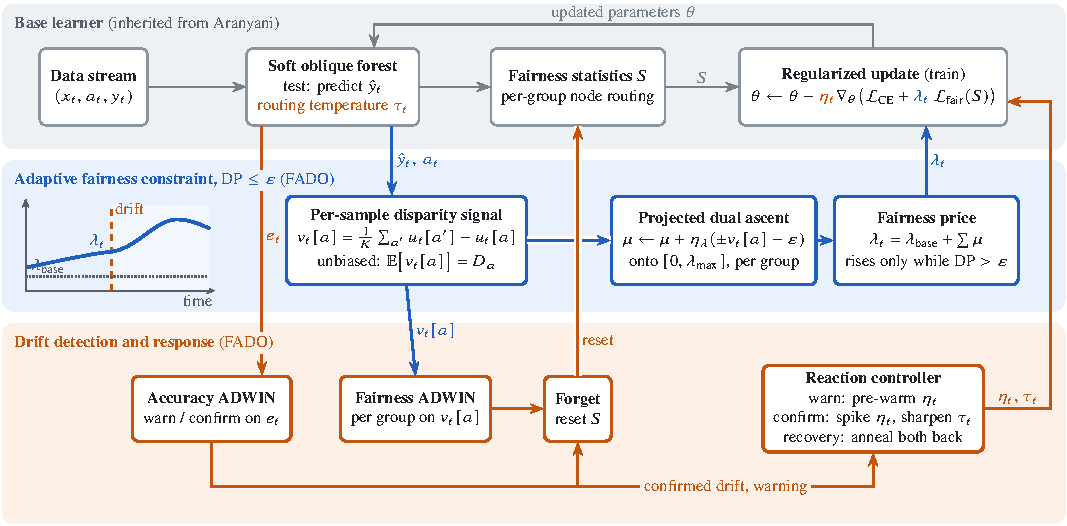
\includegraphics{figures/fado_architecture}
\caption{Overview of \fado{}. Gray: the fair soft oblique forest~\cite{chowdhury2024enhancing}, which predicts and then trains on each sample. Blue: the
adaptive fairness constraint, which turns each prediction into a disparity signal and sets the fairness price $\lambda_t$. Orange: drift detection and
response, which resets the fairness statistics $S$ on drift and adjusts the learning rate $\eta_t$ and routing temperature $\tau_t$. Colored symbols in gray
boxes are set by \fado{}.}
\label{fig:drift-pipeline}
\end{figure*}

\subsection{Forest Model}
\label{sec:method:model}
\fado{}'s predictive model is a fair soft oblique decision forest~\cite{chowdhury2024enhancing}, to which we refer for its details. It is an ensemble of $M$ soft
oblique trees of depth $h$ whose internal node $j$ routes an input to its left child with probability $n_j(x)=\sigma(w_j^{\top}x+b_j)$ and to its right
child otherwise. Fairness is imposed on these routing decisions: \ara{} constrains the deviation $F_{j,a}$ of each node's average routing decision for group $a$
from its average over all inputs (for two groups, the difference between the groups' averages), the per-node analogue of $D_a$ in~\eqref{eq:dp}, and then
relaxes the constraints into the regularized objective:
\begin{equation}
\mathcal{L}=\mathcal{L}_{\mathrm{CE}}+\lambda\,\mathcal{L}_{\text{fair}},\qquad
\mathcal{L}_{\text{fair}}=\sum_{j}\frac{1}{K}\sum_{a\in\mathcal{A}}\phi_\delta\big(F_{j,a}\big),
\label{eq:reg}
\end{equation}
where $\mathcal{L}_{\mathrm{CE}}$ is the cross-entropy loss, $\phi_\delta$ is a Huber surrogate, and $\lambda$ is a fixed hyperparameter. It estimates the
fairness gradient online from running per-group averages of the routing decisions and of their gradients, the statistics $S$, so no past sample is stored.
Our implementation, used identically by \fado{} and the \ara{} baseline, takes the cross-group mean unweighted and gives the linear branch of $\phi_\delta$ a
unit slope.

\fado{} turns this static, fixed-weight model into one (more flexible) that adapts to the stream, through three changes. First, the fixed weight $\lambda$ becomes the price $\lambda_t$ of Section~\ref{sec:method:lambda}. Second,
the statistics $S$ are reset when a drift is confirmed. Third, \fado{} adds a routing temperature, $n_j(x)=\sigma\big((w_j^{\top}x+b_j)/\tau\big)$, which
recovers \ara{} at $\tau=1$ and which the reaction controller lowers after a confirmed drift to make routing nearly hard
(Section~\ref{sec:method:drift}).

\subsection{Adaptive Fairness Constraint}
\label{sec:method:lambda}
\fado{} solves~\eqref{eq:cons} online by treating the weight $\lambda$ in~\eqref{eq:reg} as a Lagrange multiplier.

\paragraph*{One-Sided Linear Constraints}
Since $|x|\le\varepsilon$ holds exactly when $x\le\varepsilon$ and $-x\le\varepsilon$, the constraint $\mathrm{DP}\le\varepsilon$ is equivalent to the $2K$
one-sided constraints:
\begin{equation}
+D_a\le\varepsilon,\qquad -D_a\le\varepsilon,\qquad a\in\mathcal{A}.
\label{eq:onesided}
\end{equation}
The rewrite has no absolute value and no maximum, and it states \emph{which side} of the mean a group falls on. Its purpose is statistical: each constraint is
linear in $D_a$, so an unbiased estimate of $D_a$ is an unbiased estimate of every constraint's value. An absolute value would not preserve this 
($\mathbb{E}|v|\neq|\mathbb{E}v|$) and a controller fed with the magnitude of a noisy disparity estimate would read noise as unfairness and raise the price
indefinitely on a perfectly fair model.

\paragraph*{Lagrangian and Dual Ascent}
Attaching a multiplier $\mu_{a,\pm}\ge0$ to each constraint gives the Lagrangian:
\begin{equation}
\mathcal{L}(\theta,\mu)=\mathcal{L}_{\mathrm{CE}}(\theta)+\sum_{a}\Big[\mu_{a,+}(D_a-\varepsilon)+\mu_{a,-}(-D_a-\varepsilon)\Big],
\end{equation}
and~\eqref{eq:cons} is the saddle point $\min_\theta\max_{\mu\ge0}\mathcal{L}$~\cite{boyd2004convex}. The gradient of $\mathcal{L}$ in $\mu_{a,\pm}$ is the
violation $\pm D_a-\varepsilon$, so projected ascent reads:
\begin{equation}
\mu_{a,\pm}\leftarrow\Pi_{[0,\lambda_{\max}]}\big(\mu_{a,\pm}+\eta_\lambda(\pm D_a-\varepsilon)\big),
\label{eq:dual}
\end{equation}
This projection alternates with the usual gradient step in $\theta$ (primal--dual descent--ascent~\cite{mahdavi2012trading}). In control terms, $\mu$ \emph{integrates} the
violation: it keeps rising while a group's deviation exceeds $\varepsilon$ and stops only when it does not, so it has no steady-state error. 
While a group's deviation stays below $\varepsilon$, its multiplier drains toward zero, so the penalty weight decreases gradually while the stream remains fair.
The projection keeps the prices nonnegative, as duality
requires, and bounded (although it is not strictly necessary) to protect accuracy. \fado{} sums the prices into a single weight for the node-level penalty of~\eqref{eq:reg}:
\begin{equation}
\lambda_t=\min\Big(\lambda_{\mathrm{base}}+\sum_{a,\pm}\mu_{a,\pm},\ \lambda_{\max}\Big),
\label{eq:lambda}
\end{equation}
where $\lambda_{\mathrm{base}}$ is the fixed weight used by the \ara{} baseline. \fado{} therefore never applies less fairness pressure than \ara{}, and adds
pressure only while the constraint is violated. The floor is not needed by the method: with $\lambda_{\mathrm{base}}=0$, the weight is set entirely by the
prices, that is, by the constraint. We use $\lambda_{\mathrm{base}}>0$ only to make the comparison with \ara{} fair: both models start from the same weight, so
any difference in utility or fairness cannot come from a different initial penalty. Penalizing the nodes is a solid way to reduce output disparity: \ara{} shows that when every node treats the
groups alike, the demographic parity of the forest's output is bounded~\cite[Lemma~1]{chowdhury2024enhancing}.

\paragraph*{A Per-Sample Estimate of the Violation}
Online, $D_a$ is never observed: each step reveals one individual, from one group. We therefore build, from that single sample, a quantity that equals $D_a$ in
expectation. Let $\pi_a=\Pr(a_t=a)$ and define:
\begin{equation}
u_t[a]=\frac{\hat y_t\,\mathbf{1}[a_t=a]}{\pi_a},\qquad v_t[a]=\frac1K\sum_{a'}u_t[a']-u_t[a].
\label{eq:ht}
\end{equation}

\begin{proposition}[Unbiased per-sample disparity]
\label{prop:ht}
Conditional on the current model, if $(x_t,a_t)$ is drawn from the stream distribution, then $\mathbb{E}[u_t[a]]=\hat p_a$ and $\mathbb{E}[v_t[a]]=D_a$ for every
group $a$. Consequently $\pm v_t[a]-\varepsilon$ is an unbiased estimate of the violation of each constraint in~\eqref{eq:onesided}.
\end{proposition}
\begin{IEEEproof}
$u_t[a]$ is nonzero only if $a_t=a$ and $\hat y_t=1$, an event of probability $\pi_a\hat p_a$, in which case it equals $1/\pi_a$. Hence
$\mathbb{E}[u_t[a]]=\hat p_a$, the Horvitz--Thompson identity~\cite{bbbe4e97-7833-3faa-820c-4c61f82fe965}. By linearity,
$\mathbb{E}[v_t[a]]=\frac1K\sum_{a'}\hat p_{a'}-\hat p_a=D_a$. The constraints in~\eqref{eq:onesided} are linear in $D_a$, which gives the last claim.
\end{IEEEproof}

Substituting $v_t$ for $D_a$ in~\eqref{eq:dual} yields a stochastic dual ascent whose steps are correct on average. The signal needs no window, so it responds from
the first sample after a change, and successive values are conditionally independent, whereas a rolling disparity over $W$ samples is almost perfectly
autocorrelated. In practice $\pi_a$ is replaced by the running share $\hat\pi_a$ (floored at $0.02$), which makes~\eqref{eq:ht} a consistent ratio estimator.

\begin{remark}[Expected dynamics]
\label{rem:dyn}
Under a sustained violation $\Delta_{\mathrm{DP}}=\mathrm{DP}-\varepsilon>0$, the active multipliers grow by about $\eta_\lambda\Delta_{\mathrm{DP}}$ per sample;
once $\mathrm{DP}<\varepsilon$ they drain by at most $\eta_\lambda\varepsilon$ per sample, so draining is slow by design. With two groups, $D_0=-D_1$, so the
constraints in~\eqref{eq:onesided} coincide in pairs; our implementation keeps all four multipliers, which leaves the duality intact but makes the effective dual
step $2\eta_\lambda$.
\end{remark}

\subsection{Drift Detection and Reaction Controller}
\label{sec:method:drift}
The controller observes the online error stream $e_t = \mathbf{1}[\hat{y}_t \neq y_t]$ 
through two independent adaptive windowing (ADWIN)
detectors~\cite{doi:10.1137/1.9781611972771.42}: a pre-warm detector $D_w$ and a confirmation 
detector $D_c$, parameterized by significance levels $\delta_w$ and
$\delta_c<\delta_w$ (in ADWIN a larger $\delta$ is more sensitive, so the pre-warm 
detector fires first). Both are paired with a label-noise guard that excludes a
sample from triggering an event whenever an incorrect prediction is emitted with 
post-softmax confidence above $\nu$, preventing single confident-but-wrong samples
from spuriously activating the controller. A minimum of $m_0$ samples per detector 
is enforced before the first activation to avoid early-stream false positives.

When $D_w$ fires, the optimizer learning rate is multiplied by $\beta_w$, pre-warming the 
parameters for a potential change. When $D_c$ subsequently confirms a
drift, four actions are taken atomically: (i)~the learning rate is set to 
$\beta_c \cdot \eta_0$; (ii)~the routing temperature that \fado{} adds 
(Section~\ref{sec:method:model}) is set in every tree to
$\tau_{\mathrm{drift}}$, sharpening routing decisions while the ensemble refits; 
(iii)~the running fairness statistics $S$ of Section~\ref{sec:method:model} are
reset and rebuilt from post-drift samples; and (iv)~both detectors are reset and 
a cooldown of $C$ samples is enforced before a new event can fire. Recovery is
signaled when the rolling accuracy returns to the pre-drift baseline 
(estimated over the window preceding the drift) or after a timeout of $2\Delta$ samples,
after which $\tau$ is annealed back toward its steady-state value at rate $\Delta\tau$ 
per step and $\eta$ decays linearly to $\eta_0$ over $\Delta$ steps.

The two-stage design balances a confirmation-only reaction (too slow under sudden drift) 
against pre-warming without a gate (amplifies noise). The reset in
(iii) matters for the adaptive constraint: the price of Section~\ref{sec:method:lambda} 
tracks the \emph{current} disparity, but the regularizer's direction comes
from statistics accumulated since the last reset, so without forgetting a correctly 
raised price would push along the pre-drift direction. For the same reason a
\emph{fairness monitor}: one ADWIN detector per group on the per-sample signal 
$v_t[a]$ of~\eqref{eq:ht} also resets the statistics when a group's disparity
shifts; it does not change the learning rate or the temperature. Because the signal 
is unbiased and not autocorrelated, this detector avoids the false alarms that a
rolling-window disparity would cause. Concrete values for all controller parameters 
are reported in Table~\ref{tab:hparams}. Fig.~\ref{fig:alg} combines the three mechanisms into \fado{}'s prequential
test-then-train loop.

\begin{figure}[t]
\footnotesize
\begin{algorithmic}[1]
\Require stream $\{(x_t,y_t,a_t)\}$; settings of Table~\ref{tab:hparams}
\State init forest $f$, optimizer at $\eta_0$, temperature $\tau$, multipliers $\mu\gets0$, running fairness stats $S$
\For{$t = 1$ \textbf{to} $T$}
  \State $\hat{y}_t \gets \arg\max f(x_t)$;\ \ $e_t \gets \mathbf{1}[\hat{y}_t \neq y_t]$ \Comment{test}
  \State update windowed accuracy, DP, and EO over the last $W$ samples
  \State $\textit{noise} \gets e_t \wedge (\text{conf}(\hat{y}_t) > \nu)$ \Comment{label-noise guard}
  \State $\textit{ok} \gets \neg\textit{noise} \wedge (t-t_{\text{last}}\geq C)$ \Comment{guard, cooldown}
  \If{$D_w(e_t)$ warns \textbf{and} \textit{ok}} $\eta \gets \beta_w\,\eta_0$ \Comment{pre-warm} \EndIf
  \If{$D_c(e_t)$ confirms \textbf{and} \textit{ok}}
     \State $\eta \gets \beta_c\,\eta_0$;\ $\tau \gets \tau_{\mathrm{drift}}$;\ reset $S$;\ $t_{\text{last}}\gets t$ \Comment{spike + sharpen}
  \EndIf
  \State compute $v_t[a]$ by~\eqref{eq:ht}; reset $S$ if a fairness detector confirms
  \State $\mu_{a,\pm} \gets \Pi_{[0,\lambda_{\max}]}\big(\mu_{a,\pm} + \eta_\lambda(\pm v_t[a]-\varepsilon)\big)$ \Comment{dual ascent}
  \State $\lambda_t \gets \min(\lambda_{\mathrm{base}}+\sum\mu,\ \lambda_{\max})$
  \State \textbf{if} recovered \textbf{or} timed out \textbf{then} anneal $\eta\!\to\!\eta_0$ over $\Delta$, $\tau\!\to\!1$
  \State accumulate $(x_t,y_t,a_t)$ into $S$ \Comment{train}
  \State optimizer step on $\nabla\big(\mathcal{L}_{\mathrm{CE}}(f(x_t),y_t) + \lambda_t\,\mathcal{L}_{\mathrm{fair}}(S)\big)$ at rate $\eta$
\EndFor
\end{algorithmic}
\caption{\fado{}'s prequential test-then-train loop. Available at [undisclosed for blind review].}
\label{fig:alg}
\end{figure}

\subsection{Datasets and Preprocessing}
\label{sec:method:data}
Table~\ref{tab:datasets} summarizes the two datasets. \folk{} (ACS Income, CA)~\cite{ding2022retiringadultnewdatasets} supplies a large natural cross-year shift between 2015
(training) and 2017--2018 (prequential test); \adult{}~\cite{adult_2} provides a controlled testbed on which we inject concept-drift perturbations of a
known form on the test stream. Both datasets are processed through a shared tabular pipeline: numerical features are standardized using training-set means and
standard deviations, and categorical variables are one-hot encoded. The encoder is fitted on the training split alone and reused unchanged for the test stream, so
the streaming protocol remains free of test-time information leakage.

\begin{table}[t]
\centering
\caption{Datasets}
\label{tab:datasets}
\setlength{\tabcolsep}{1.5pt}
\footnotesize
\begin{tabular}{@{}L{1.6cm} L{1.25cm} L{1.05cm} L{1.15cm} L{2.5cm}@{}}
\toprule
Dataset & Size & Target & Protected attribute & Split / stream \\
\midrule
\folk{} (ACS Income, CA) & 187{,}474 + \newline 187{,}475 & Income $>$ \$50k & Sex (2 groups) & Train 2015; test 2017--2018 in temporal order; both splits uniformly subsampled to 10\% per seed \\
\adult{} & 32{,}561 + \newline 16{,}281 & Income $>$ \$50k & Sex (2 groups) & Standard train/test split; one injected drift per test stream \\
\bottomrule
\end{tabular}
\end{table}

\subsection{Concept-Drift Scenarios}
\label{sec:method:scenarios}
We adopt complementary strategies on the two datasets. On \folk{}, training on 2015 
and evaluating prequentially on 2017--2018 already provides a real,
multidimensional cross-year shift driven by genuine demographic and economic change; 
injecting additional synthetic perturbations on top of it would mask
controlled and natural signals obscuring the source of any observed degradation.

On \adult{} the test stream carries no known drift, so we inject it. 
Following the benchmarking framework of Cerqueira et al.~\cite{10.1145/3770855.3819070}, which injects 
controlled distributional changes into real-world datasets to evaluate drift detectors, we use its four drift types, 
each giving a separate scenario: every model ran on all four, with one drift per stream at an onset drawn uniformly between $50\%$ 
and $70\%$ of the stream. The four types are \emph{x\_permutations}, where the feature vector 
is permuted by a fixed random permutation, changing the mapping from inputs to labels;
\emph{y\_swaps}, where samples of one randomly chosen class are relabeled with probability $0.5$, 
a concept drift in $P(y\mid x)$; \emph{y\_prior\_skip}, where
$75\%$ of the samples of one class are dropped, a prior shift; and \emph{x\_exceed\_skip}, 
where samples whose value of a randomly chosen numerical feature exceeds
its training median are dropped, a covariate shift. The onset, the drifted class, the 
permutation, and the feature are drawn from the seed, so each seed is a
different stream; the order of the \adult{} test split is fixed.

\subsection{Baselines}
\label{sec:method:baselines}
We compare \fado{} against three streaming baselines that span the 
accuracy/fairness/adaptivity design space, and against an optimistic variant of the third:
\begin{itemize}
\item \textbf{\arf{}}~\cite{10.1007/s10994-017-5642-8}: the Adaptive Random Forest 
from the River library~\cite{montiel2020rivermachinelearningstreaming}, used as an accuracy-oriented
streaming reference that handles drift through per-tree warning and drift detectors 
and background trees, but without any fairness mechanism;
\item \textbf{\rfr{}}: a sharpness-aware reweighting variant that applies the \rfr{} 
optimizer~\cite{jiang2023chasingfairnessdistributionshift} (sharpness-aware
minimization over a fairness-reweighted loss); this provides a fairness-aware static 
baseline without adaptive drift handling;
\item \textbf{\ara{}}~\cite{chowdhury2024enhancing}: the plain \ara{} forest, with the fixed weight $\lambda=0.1$ of its published configuration and
no drift handling;
\item \textbf{\ara{} with leaked $\lambda$}: the same forest given a constant weight of at least \fado{}'s mean $\lambda_t$ on each dataset ($0.5$ on \folk{}
and $1.5$ on \adult{}), a value we read off \fado{}'s own runs, and pre-trained with $\lambda_{\mathrm{base}}=0.1$ like \fado{}, so that both start from the same
forest. A fixed-weight learner has no way to arrive at this value by itself: it could only obtain it by tuning $\lambda$ separately for every dataset, whereas
\fado{} reaches it online, without tuning. The leaked weight therefore gives \ara{} an advantage it would not have in practice; we include this baseline to
separate the benefit of a larger weight from the benefit of adapting it.
\end{itemize}
All methods are evaluated under the same test-then-train prequential protocol with batch size~$1$ as \fado{} so that comparisons are not biased by data ordering
or data leakage. The global random number generators (NumPy, 
Python \texttt{random}, and TensorFlow) are pinned per seed and TensorFlow op
determinism is enabled, so the data split, the forest initialization, and the 
training trajectory are identical across methods that share a seed.

\subsection{Hyperparameter Selection}
\label{sec:method:hpo}
Table~\ref{tab:hparams} lists the fairness and controller hyperparameters with 
their \adult{} defaults and the \folk{} overrides. For the forest we keep the
settings of~\cite{chowdhury2024enhancing}: $M=3$ trees of depth $h=4$, trained with 
Adam at $\eta_0=2{\times}10^{-3}$. The remaining values were set before the reported 
runs and were never tuned on the reporting seeds. 

As argued in Section~\ref{sec:problem:constraint}, the fairness target $\varepsilon=0.05$ is a fixed requirement rather 
than a tuned value: for two groups it allows a positive-prediction-rate
gap of at most $0.10$. The dual step $\eta_\lambda=0.01$ trades responsiveness against 
noise in the per-sample signal (Remark~\ref{rem:dyn}), and the cap
$\lambda_{\max}=10$ bounds the accuracy that the price can spend when $\varepsilon$ is 
hard to reach; the cap is not required by the method. The surrogate transition is $\delta=0.1$, larger than the
$0.01$ used in~\cite{chowdhury2024enhancing}.

The two ADWIN levels make the warning detector fire first: in ADWIN a larger $\delta$ is 
more sensitive, so $\delta_w=2{\times}10^{-2}$ gives an early warning,
while $\delta_c=10^{-5}$ requires a strong, sustained rise of the error rate before the 
full reaction starts. The learning-rate multipliers $\beta_w{=}5$ and
$\beta_c{=}10$ keep a $1{:}2$ ratio: a warning gives a measurable pre-warm without committing 
the model to a new regime, and only a confirmed drift triggers the
full spike. The drift temperature $\tau_{\mathrm{drift}}=0.1$, ten times lower than the 
steady-state $\tau=1$, makes routing nearly hard during the spike, so the
forest can move to a new leaf assignment within a few dozen samples instead of waiting 
for the soft routing weights to average over the new regime. The anneal
$\Delta\tau=2{\times}10^{-3}$ returns $\tau$ from $0.1$ to $1$ in $450$ steps, well 
inside the $\Delta=3000$ learning-rate decay horizon. The cooldown $C=200$
stops the controller from firing again during its own response, and the label-noise 
guard $\nu=0.7$ keeps wrong predictions from triggering
an event. Because \folk{}'s drift is a gradual change between survey years rather 
than an abrupt break, we fixed a milder reaction for it in advance: a smaller
spike ($\beta_c=3$), a softer temperature ($\tau_{\mathrm{drift}}=0.5$), and a 
shorter horizon ($\Delta=1000$), which avoid overreacting to a slow change.

\begin{table}[t]
\centering
\caption{\fado{} Hyperparameters}
\label{tab:hparams}
\setlength{\tabcolsep}{3pt}
\footnotesize
\begin{tabular}{@{}l c c L{3.9cm}@{}}
\toprule
Symbol & \adult{} & \folk{}$^{\mathrm{a}}$ & Role \\
\midrule
\multicolumn{4}{@{}l}{{Fairness regularizer and constraint}} \\
$\lambda_{\mathrm{base}}$ & $0.1$ & -- & floor of $\lambda_t$; \ara{}'s fixed $\lambda$ \\
$\varepsilon$ & $0.05$ & -- & demographic-parity target \\
$\eta_\lambda$ & $0.01$ & -- & dual step size \\
$\lambda_{\max}$ & $10$ & -- & cap on $\lambda_t$ \\
$\delta$ & $0.1$ & -- & quadratic/linear transition in $\phi_\delta$ \\
$W$ & $1000$ & -- & rolling window for reported metrics \\
\midrule
\multicolumn{4}{@{}l}{{Drift detection and reaction controller}} \\
$\delta_w$ & $2\times10^{-2}$ & -- & ADWIN significance (pre-warm) \\
$\delta_c$ & $1\times10^{-5}$ & -- & ADWIN significance (confirmation) \\
$\delta_{\mathrm{fair}}$ & $2\times10^{-3}$ & -- & ADWIN significance (fairness monitor) \\
$\beta_w$ & $5$ & -- & learning-rate multiplier on warning \\
$\beta_c$ & $10$ & $3$ & learning-rate multiplier on confirmed drift \\
$\Delta$ & $3000$ & $1000$ & learning-rate decay horizon back to $\eta_0$ \\
$\tau$ & $1.0$ & -- & steady-state routing temperature (added by \fado{}) \\
$\tau_{\mathrm{drift}}$ & $0.1$ & $0.5$ & temperature set on confirmed drift \\
$\Delta\tau$ & $2\times10^{-3}$ & -- & per-step temperature anneal back to $\tau$ \\
$C$ & $200$ & -- & cooldown (samples) between events \\
$\nu$ & $0.7$ & -- & label-noise confidence guard \\
$m_0$ & $30$ & -- & minimum samples before first activation \\
\bottomrule
\end{tabular}
\tnote{$^{\mathrm{a}}$A dash means the \folk{} value equals the \adult{} value.}
\end{table}

\subsection{Evaluation Protocol}
\label{sec:method:protocol}
All methods are evaluated under a strict prequential test-then-train protocol with batch size~$1$~\cite{10.1007/s10994-012-5320-9}: at each step the model emits
$\hat{y}_t$, the prequential metrics are updated, and only then is the parameter update 
performed using the just-observed $(y_t, a_t)$. We report mean and
standard deviation over $30$ reporting seeds, disjoint from the 
seeds used during development. The primary metrics are the F1 score of the positive class
and the demographic-parity violation, with equalized odds as a secondary, unoptimized 
criterion. Each is reported over the whole stream and over the part of the stream after the injected onset: DP and EO are
computed over the same $W$-sample rolling window and averaged over that part, and F1 is computed from all its predictions.

All experiments ran on CPU, in Python~3.11 or~3.12, on three machines: a Linux workstation with an Intel Core i9-9900K, a Windows desktop with an Intel
Core i5-8500, and an Apple M5 laptop. Each run executes all the methods of its sweep for one seed on one machine, so every paired comparison
below is made on the same stream. A seed's stream is the same on every machine, and so are the results of \fado{} and of both
\ara{} variants: before the onset, the four \adult{} scenarios of a seed share the same stream, and these methods' per-seed metrics on it are identical across
scenarios that ran on different machines. \arf{} and \rfr{} are reproducible on each machine but differ slightly across machines (a seed's demographic
parity before the onset by at most $0.010$).

For each metric column, paired-by-seed comparisons of \fado{} against each other method are 
performed using the two-sided Wilcoxon signed-rank test; $p$-values are
corrected within each column of each block using the Holm--Bonferroni step-down procedure across the 
four methods compared with \fado{} (Section~\ref{sec:method:baselines}). As a stricter
check, we also apply the correction across all the comparisons of Table~\ref{tab:results} at once. The procedure follows the recommendations of
Dem{\v{s}}ar~\cite{demsar2006statistical}. We prefer the paired Wilcoxon test to the Welch two-sample $t$-test because it assumes no distribution for the
per-seed metric and uses the pairing given by the shared data ordering (Section~\ref{sec:method:baselines}), which Welch ignores. The Welch results are reported
alongside in the repository (Section~\ref{sec:method:reproducibility}).

\subsection{Reproducibility}
\label{sec:method:reproducibility}
The full implementation, configuration files, seed manifests, and per-seed result files 
are released at [undisclosed for blind review]. The repository lists the sweep configuration
behind every reported run; one script regenerates Tables~\ref{tab:results} and~\ref{tab:detection} and the full significance report (paired
Wilcoxon and Welch tests, raw and Holm-corrected $p$-values) from the per-seed results, and a second script recomputes, with its
derivation, every number quoted in the text.

% =====================================================================
\section{Results and Discussion}
\label{sec:results}

% Generated by scripts/make_tables.py -- edit the script, not this table.
\begin{table*}[t]
\centering
\caption{F1, Demographic Parity, and Equalized Odds Over 30 Seeds, Whole Stream and After the Drift Onset$^{\mathrm{a}}$}
\label{tab:results}
\setlength{\tabcolsep}{4pt}
\footnotesize
\begin{tabular}{@{}l ccc ccc@{}}
\toprule
& \multicolumn{3}{c}{Whole stream} & \multicolumn{3}{c}{After onset$^{\mathrm{c}}$} \\
\cmidrule(lr){2-4} \cmidrule(l){5-7}
Method & F1$^{\mathrm{b}}$\,$\uparrow$ & DP\,$\downarrow$ & EO\,$\downarrow$ & F1$^{\mathrm{b}}$\,$\uparrow$ & DP\,$\downarrow$ & EO\,$\downarrow$ \\
\midrule
\multicolumn{7}{@{}l}{{\folk{}, natural cross-year shift}} \\
\fado{} & $0.758\pm 0.005$ & $0.042\pm 0.003\sig{***}$ & $0.025\pm 0.003\sig{***}$ & n/a & n/a & n/a \\
\ara{} & $\mathbf{0.762\pm 0.005}$ & $0.057\pm 0.004$ & $0.036\pm 0.003$ & n/a & n/a & n/a \\
\ara{}, leaked $\lambda^{\mathrm{d}}$ & $0.759\pm 0.005$ & $\mathbf{0.039\pm 0.004}^{\dagger}$ & $\mathbf{0.024\pm 0.003}^{\dagger}$ & n/a & n/a & n/a \\
\arf{} & $0.640\pm 0.009$ & $0.072\pm 0.012$ & $0.077\pm 0.016$ & n/a & n/a & n/a \\
\rfr{} & $0.729\pm 0.005$ & $0.075\pm 0.006$ & $0.059\pm 0.006$ & n/a & n/a & n/a \\
\midrule
\multicolumn{7}{@{}l}{{\adult{}, x\_permutations}} \\
\fado{} & $0.612\pm 0.010$ & $\mathbf{0.060\pm 0.004}\sig{***}$ & $\mathbf{0.053\pm 0.009}\sig{***}$ & $0.550\pm 0.029$ & $\mathbf{0.062\pm 0.010}\sig{***}$ & $\mathbf{0.064\pm 0.022}\sig{***}$ \\
\ara{} & $0.609\pm 0.019$ & $0.083\pm 0.007$ & $0.073\pm 0.010$ & $0.513\pm 0.056$ & $0.085\pm 0.014$ & $0.115\pm 0.025$ \\
\ara{}, leaked $\lambda^{\mathrm{d}}$ & $0.590\pm 0.021^{\dagger}$ & $0.062\pm 0.009$ & $0.070\pm 0.013^{\dagger}$ & $0.493\pm 0.063^{\dagger}$ & $0.077\pm 0.018^{\dagger}$ & $0.100\pm 0.028^{\dagger}$ \\
\arf{} & $0.571\pm 0.011$ & $0.090\pm 0.003$ & $0.110\pm 0.013$ & $0.519\pm 0.026$ & $0.086\pm 0.006$ & $0.119\pm 0.026$ \\
\rfr{} & $\mathbf{0.626\pm 0.006}$ & $0.100\pm 0.004$ & $0.091\pm 0.010$ & $\mathbf{0.613\pm 0.010}$ & $0.102\pm 0.007$ & $0.104\pm 0.019$ \\
\midrule
\multicolumn{7}{@{}l}{{\adult{}, y\_swaps}} \\
\fado{} & $0.645\pm 0.058$ & $\mathbf{0.048\pm 0.004}\sig{***}$ & $\mathbf{0.048\pm 0.006}\sig{**}$ & $0.526\pm 0.222$ & $\mathbf{0.027\pm 0.011}\sig{***}$ & $\mathbf{0.052\pm 0.013}\sig{*}$ \\
\ara{} & $\mathbf{0.647\pm 0.047}$ & $0.071\pm 0.010$ & $0.056\pm 0.010$ & $0.524\pm 0.206$ & $0.054\pm 0.028$ & $0.069\pm 0.024$ \\
\ara{}, leaked $\lambda^{\mathrm{d}}$ &  &  &  &  &  &  \\
\arf{} & $0.615\pm 0.063$ & $0.084\pm 0.005$ & $0.096\pm 0.011$ & $\mathbf{0.561\pm 0.164}$ & $0.072\pm 0.014$ & $0.083\pm 0.017$ \\
\rfr{} & $0.635\pm 0.063$ & $0.089\pm 0.015$ & $0.084\pm 0.015$ & $0.504\pm 0.245$ & $0.072\pm 0.039$ & $0.083\pm 0.037$ \\
\midrule
\multicolumn{7}{@{}l}{{\adult{}, y\_prior\_skip}} \\
\fado{} & $0.676\pm 0.051$ & $0.059\pm 0.011\sig{***}$ & $\mathbf{0.049\pm 0.008}\sig{**}$ & $0.621\pm 0.229$ & $\mathbf{0.063\pm 0.042}\sig{***}$ & $\mathbf{0.054\pm 0.023}\sig{**}$ \\
\ara{} & $\mathbf{0.695\pm 0.049}$ & $0.083\pm 0.017$ & $0.054\pm 0.006$ & $\mathbf{0.667\pm 0.201}$ & $0.097\pm 0.066$ & $0.076\pm 0.018$ \\
\ara{}, leaked $\lambda^{\mathrm{d}}$ & $0.679\pm 0.053^{\dagger}$ & $\mathbf{0.058\pm 0.015}$ & $0.056\pm 0.011^{\dagger}$ & $0.656\pm 0.206^{\dagger}$ & $0.079\pm 0.057^{\dagger}$ & $0.067\pm 0.025^{\dagger}$ \\
\arf{} & $0.631\pm 0.059$ & $0.091\pm 0.022$ & $0.093\pm 0.019$ & $0.522\pm 0.305$ & $0.106\pm 0.078$ & $0.089\pm 0.044$ \\
\rfr{} & $0.671\pm 0.058$ & $0.099\pm 0.021$ & $0.084\pm 0.012$ & $0.629\pm 0.240$ & $0.112\pm 0.076$ & $0.092\pm 0.031$ \\
\midrule
\multicolumn{7}{@{}l}{{\adult{}, x\_exceed\_skip}} \\
\fado{} & $0.633\pm 0.016$ & $\mathbf{0.057\pm 0.005}\sig{***}$ & $0.048\pm 0.007$ & $0.576\pm 0.080$ & $\mathbf{0.049\pm 0.013}\sig{***}$ & $0.051\pm 0.018$ \\
\ara{} & $\mathbf{0.647\pm 0.016}$ & $0.076\pm 0.007$ & $\mathbf{0.047\pm 0.006}$ & $\mathbf{0.594\pm 0.077}$ & $0.061\pm 0.017$ & $\mathbf{0.047\pm 0.015}$ \\
\ara{}, leaked $\lambda^{\mathrm{d}}$ &  &  &  &  &  &  \\
\arf{} & $0.586\pm 0.022$ & $0.083\pm 0.006$ & $0.090\pm 0.013$ & $0.502\pm 0.122$ & $0.065\pm 0.020$ & $0.076\pm 0.016$ \\
\rfr{} & $0.620\pm 0.016$ & $0.093\pm 0.005$ & $0.081\pm 0.010$ & $0.560\pm 0.088$ & $0.076\pm 0.020$ & $0.074\pm 0.020$ \\
\bottomrule
\end{tabular}
\tnote{$^{\mathrm{a}}$Mean $\pm$ standard deviation over 30 seeds. Bold marks the best mean per
metric within each block. Superscripts on \fado{} mark a paired Wilcoxon test, Holm-corrected, significant in \fado{}'s favor against each of \ara{}, \arf{}, and \rfr{}
($^{*}p<0.05$, $^{**}p<0.01$, $^{***}p<0.001$); columns with no marker have mixed per-baseline directions and are dissected in the text.
$^{\mathrm{b}}$F1 of the positive class (income $>$ \$50k), computed from the per-sample predictions (one confusion matrix per run and part of the stream). Empty cells: not yet computed.
$^{\mathrm{c}}$From the injected drift onset to the end of the test stream (the drifted part of the stream); DP and EO are the rolling-window values averaged over that part. \folk{} has no injected onset (n/a).
$^{\mathrm{d}}$\ara{} with a constant $\lambda$ chosen after the fact from \fado{}'s own runs, at least \fado{}'s mean $\lambda_t$ on that dataset ($0.5$ on \folk{}, $1.5$ on \adult{}). This gives the baseline an advantage it would not have in practice, the value of $\lambda$ leaked from \fado{}, so it is the strongest fixed-$\lambda$ \ara{} we can construct. It is pre-trained with $\lambda_{\mathrm{base}}=0.1$, like \fado{}, so both start from the same forest. $^{\dagger}$Significantly different from \fado{} (paired two-sided Wilcoxon test, $p<0.05$); bold shows which is better. Empty rows: runs not finished.}
\end{table*}

% Generated by scripts/make_tables.py -- edit the script, not this table.
\begin{table}[t]
\centering
\caption{Overall Comparison of \fado{} Against Each Method}
\label{tab:overall}
\setlength{\tabcolsep}{4pt}
\footnotesize
\begin{tabular}{@{}l ccc@{}}
\toprule
& Significant & No significant & Significant \\
\fado{} vs. & wins & difference & losses \\
\midrule
\ara{} & 17 & 5 & 5 \\
\ara{}, leaked $\lambda$ & 12 & 8 & 7 \\
\arf{} & 26 & 1 & 0 \\
\rfr{} & 24 & 0 & 3 \\
\midrule
Total (108) & 79 & 14 & 15 \\
\bottomrule
\end{tabular}
\tnote{Counts over the 27 cells of each method in Table~\ref{tab:results} (paired Wilcoxon test, Holm-corrected, $\alpha=0.05$).}
\end{table}

% Generated by scripts/make_tables.py -- edit the script, not this table.
\begin{table*}[t]
\centering
\caption{Detection of the Injected Drift by \fado{} on \adult{}, 30 Seeds per Scenario$^{\mathrm{a}}$}
\label{tab:detection}
\setlength{\tabcolsep}{5pt}
\footnotesize
\begin{tabular}{@{}l cc cc cc cc@{}}
\toprule
& \multicolumn{2}{c}{Either detector} & \multicolumn{2}{c}{Accuracy detector} & \multicolumn{2}{c}{Fairness monitor} & \multicolumn{2}{c}{False alarms per run$^{\mathrm{c}}$} \\
\cmidrule(lr){2-3} \cmidrule(lr){4-5} \cmidrule(lr){6-7} \cmidrule(l){8-9}
Scenario & Detected & Delay$^{\mathrm{b}}$ & Detected & Delay$^{\mathrm{b}}$ & Detected & Delay$^{\mathrm{b}}$ & Accuracy & Fairness \\
\midrule
x\_permutations & 13/30 (43\%) & $505$ & 11/30 (37\%) & $426$ & 2/30 (7\%) & $943$ & $0.17$ & $0.83$ \\
y\_swaps & 16/30 (53\%) & $116$ & 16/30 (53\%) & $116$ & 3/30 (10\%) & $675$ & $0.13$ & $1.83$ \\
y\_prior\_skip & 27/30 (90\%) & $535$ & 10/30 (33\%) & $781$ & 17/30 (57\%) & $390$ & $0.47$ & $1.43$ \\
x\_exceed\_skip & 2/30 (7\%) & $866$ & 0/30 (0\%) & -- & 2/30 (7\%) & $866$ & $0.17$ & $0.40$ \\
\midrule
All & 58/120 (48\%) & $424$ & 37/120 (31\%) & $388$ & 24/120 (20\%) & $511$ & $0.23$ & $1.12$ \\
\bottomrule
\end{tabular}
\tnote{$^{\mathrm{a}}$An onset counts as detected when the detector raises an alarm within $1{,}000$ samples after it, the length of one rolling window: a window-based detector cannot register a change before its window has refilled, so a later alarm is no longer attributed to the injected drift. \emph{Either detector} counts a run once if the accuracy detector or the fairness monitor detects the onset; \folk{} has no injected onset and is not scored.
$^{\mathrm{b}}$Mean number of samples from the onset to the first alarm within that window, over the detected runs only; by construction it is at most $1{,}000$, so it must be read together with the detection rate.
$^{\mathrm{c}}$Alarms not matched to the onset, averaged over the 30 runs; every alarm of the fairness monitor, matched or not, resets the penalty's running statistics.}
\end{table*}

% The split of Table~\ref{tab:detection} by detected / undetected runs (FADO minus
% Aranyani after the onset) is in supplementary/detection_split.md, to be published
% with the repository; ICDE allows no appendix. Cite it from the Results text.

Table~\ref{tab:results} reports F1, demographic parity (DP), and equalized odds (EO) as mean $\pm$ standard deviation over the $30$ seeds, which all methods
share, both over the whole stream and over the part of each \adult{} stream that follows the injected onset; \folk{} has no onset because its shift lies between the
training year and the test stream. We measure utility with the F1 score of the positive class (income above \$50k) because that class is a minority:
$40\%$ of the \folk{} stream and $24\%$ of the \adult{} test split. Bold marks the best mean of each metric within a block. The column $\lambda$ gives
the fairness weight over the whole stream: for \fado{}, the mean of $\lambda_t$; for the two \ara{} variants, their constant weight.

Every value of the other methods in Table~\ref{tab:results} carries the outcome of its paired test against \fado{} (Section~\ref{sec:method:protocol}): $^{\bullet}$
if \fado{} is significantly better, $^{\circ}$ if it is significantly worse, and no mark if no significant difference is detected, which does not establish that the two
are equivalent. Table~\ref{tab:overall} sums these outcomes over the $27$ cells of each method: $3$ metrics in $5$ blocks over the whole stream and in $4$ after the
onset. Over the $108$ comparisons, \fado{} is significantly better in $73\%$ and significantly worse in $14\%$; $73\%$ of these losses are on F1, and the
remaining $27\%$, on DP or EO, are all against \ara{} with leaked $\lambda$. With the Holm correction applied across all $108$ comparisons at once, $86\%$ of the
significant differences remain significant.

Table~\ref{tab:detection} reports how often, and how fast, \fado{}'s detectors register each injected drift. An onset counts as detected when a detector raises an
alarm within $1{,}000$ samples after it, the length of one rolling window: a window-based detector cannot register a change before its window has refilled, so a later
alarm is no longer attributed to the injected drift. The delay is the mean number of samples from the onset to that alarm over the detected runs only, so it must be
read together with the detection rate; alarms not matched to an onset count as false alarms.

We now use these results to answer the two research questions.

\subsection{To What Extent Does Concept Drift Affect Group Fairness?}
\label{sec:results:rq1}
Not every type of concept drift affects group fairness the same way: the effect depends on the type of drift and on the fairness criterion. We measure it on \adult{},
where the onset is known, by comparing each method's metrics before and after the onset on the same seeds. For the controller-free \ara{}, the drifts that alter the
relation between inputs and labels widen the gap in error rates between groups: equalized odds rises from $0.047$ to $0.115$ after the onset of
\emph{x\_permutations} (an increase on all $30$ seeds) and from $0.047$ to $0.076$ under \emph{y\_prior\_skip}, where demographic parity also rises, from $0.082$
to $0.097$. Demographic parity, in contrast, falls after the onset of \emph{y\_swaps} ($0.082$ to $0.054$), although equalized odds rises there too ($0.047$
to $0.069$), and after the onset of \emph{x\_exceed\_skip} ($0.082$ to $0.061$): relabeling one class or removing the samples above a feature's median also brings
the groups' positive-prediction rates closer. For \arf{} and \rfr{} as well, demographic parity falls after the onset of
\emph{y\_swaps} and \emph{x\_exceed\_skip}, and it remains higher than \fado{}'s before and after every onset. A fairness guarantee on
the stream before a drift is, therefore, not preserved after it and the metric that worsens can't be known in advance. This is the setting the adaptive
constraint targets.

On \folk{} the shift lies between the training year and the whole test stream, so the stream offers no reference before the drift; every method shows a slightly
lower demographic parity on the 2018 half of the stream than on the 2017 half, and we use \folk{} to assess the methods under a natural, gradual shift rather than to
measure the effect of drift itself.

\subsection{Can Adaptive Mechanisms Preserve Fairness While Maintaining Utility?}
\label{sec:results:rq2}
\textbf{Fairness against the published baselines.} In every block of Table~\ref{tab:results}, \fado{} attains a significantly lower demographic parity than
each of \ara{}, \arf{}, and \rfr{} ($p<0.001$); relative to \ara{}, the reduction ranges from $25\%$ (\emph{x\_exceed\_skip}) to $33\%$ (\emph{y\_swaps}). \fado{}'s
constraint targets demographic parity only; equalized odds is not part of its objective. Even so, \fado{}'s equalized odds is lower than that of \ara{},
\arf{}, and \rfr{} in four of the five blocks. In the fifth, \emph{x\_exceed\_skip}, it is still lower than that of \arf{} and \rfr{}, and level with
that of \ara{} ($0.048$ against $0.047$, a difference that is not significant).
The advantage also holds after the onset. In all four \adult{} scenarios, \fado{} has the lowest demographic parity of the five methods, significantly
lower than that of \ara{}, \arf{}, and \rfr{} ($p<0.001$). It also has the lowest equalized odds after the onset in three of the four scenarios; in
\emph{x\_exceed\_skip}, \ara{} is slightly lower ($0.047$ against $0.051$), but not significantly.
\fado{} also limits the increases identified in Section~\ref{sec:results:rq1}: after the onset of \emph{x\_permutations}, its equalized odds rises from $0.047$ to
$0.064$, against $0.115$ for \ara{}, and under \emph{y\_prior\_skip} its increase is not significant.

\textbf{Utility.} The fairness gain comes at a small utility cost relative to \ara{}. \fado{}'s F1 is $0.758$ against $0.762$ on \folk{} and is lower on three of
the four \adult{} drifts, by at most $0.019$ (\emph{y\_prior\_skip}); on \emph{x\_permutations} \fado{} exceeds \ara{} ($0.612$ against $0.609$), and \rfr{} attains the highest F1. \fado{}
remains well above \arf{} in every block. The cost is largest after the onset of \emph{y\_prior\_skip} ($0.621$ against $0.667$), the drift after which
\fado{} raises its fairness weight the most (to $3.01$ on average).

\textbf{Against the leaked weight.} Since \fado{}'s mean $\lambda_t$ exceeds the published weight of \ara{}, part of its fairness gain could come from a larger
weight rather than from its adaptation. The comparison with \ara{} with leaked $\lambda$, pre-trained like \fado{} so that both start from the same forest,
separates the two effects, under conditions that favor the baseline: it is given the weight that \fado{} found on that very dataset. Under \emph{x\_permutations}, \fado{} outperforms it after the onset on every metric: demographic parity $0.062$ against
$0.077$, equalized odds $0.064$ against $0.100$, and F1 $0.550$ against $0.493$. A constant weight applies more pressure than needed before the drift and less than
needed after it, which an adaptive weight avoids: \fado{}'s weight averages $0.97$ before the onset and $2.30$ after it, against the constant $1.5$. Under the other drifts the two are close and trade metrics: the leaked weight attains a lower whole-stream
demographic parity under \emph{y\_swaps} ($0.044$ against $0.048$) and \emph{x\_exceed\_skip} ($0.053$ against $0.057$), while \fado{} attains a lower equalized odds
under \emph{y\_swaps} and \emph{y\_prior\_skip}, and a lower demographic parity after the onset of \emph{y\_prior\_skip} ($0.063$ against $0.079$) at a lower F1. On the gradual
shift of \folk{}, the leaked weight is slightly fairer ($0.039$ against $0.042$ in demographic parity) at the same F1. Adapting the weight online thus matches a fixed
weight that could only have been obtained by tuning on each dataset, and improves on it under abrupt concept drift.

\textbf{Drift detection.} \fado{} detects the injected drift within one window in $48\%$ of the \adult{} runs (Table~\ref{tab:detection}). The two detectors are
complementary: the accuracy detector registers label swaps within about $116$ samples, whereas class-prior shifts are mostly registered by the fairness monitor,
which raises the detection rate on \emph{y\_prior\_skip} to $90\%$. The covariate shift of \emph{x\_exceed\_skip}, which barely affects the error rate, is detected in only
$7\%$ of the runs, and the fairness monitor raises $1.12$ unmatched alarms per run, each of which resets the penalty's running statistics. The fairness gain does not depend on
detection: in the $62$ runs where neither detector fired, \fado{}'s demographic parity after the onset remains lower than \ara{}'s in $61$, although by less than in
detected runs ($-0.013$ against $-0.035$), while its equalized-odds advantage largely requires a detection. The per-scenario split is provided with the
code (Section~\ref{sec:method:reproducibility}).

\subsection{Ablation of the Adaptive Constraint}
\label{sec:results:ablation}
To isolate the adaptive fairness constraint, we ran on \folk{}, on the same $30$ seeds as Table~\ref{tab:results}, a variant of \fado{} that keeps the drift detector and the reaction controller but uses the fixed weight
$\lambda=\lambda_{\mathrm{base}}$, without the fairness monitor and the reset. Removing these components worsens every metric on at least $28$ of the $30$ seeds
($p<10^{-8}$): demographic parity rises from $0.042$ to $0.050$, equalized odds from $0.025$ to $0.035$, and F1 falls from $0.758$ to $0.748$. The adaptive
constraint therefore improves fairness and utility together on this dataset. The gain is concentrated in the first half of the test stream (2017); on the 2018 half the
two variants reach a similar demographic parity. A per-component ablation on \adult{} is left for future work.

% =====================================================================
\section{Conclusion and Future Work}
\label{sec:conclusion}
This paper studied group fairness in online learning under concept drift and proposed \fado{}, which turns the fixed fairness weight of a fair oblique forest
into the dual price of a demographic-parity bound, tracked online from an unbiased per-sample estimate of each group's disparity, and couples it with drift
detection, a fairness monitor, and a reaction controller.

Regarding RQ1, concept drift does not degrade fairness uniformly. On \adult{}, the drifts that change the relation between inputs and labels widened the
error-rate gap of the fixed-weight learner, whose equalized odds rose from $0.047$ to $0.115$ after the feature permutation, whereas relabeling one class or
removing part of the input space narrowed its demographic parity. A fairness level calibrated before a drift is therefore not guaranteed after it, and which
criterion deteriorates depends on the drift. Regarding RQ2, \fado{} lowered demographic parity by $25$ to $33\%$ relative to the fixed-weight \ara{} in every block
and was significantly fairer in demographic parity than each of the three published baselines in all $27$ comparisons, over the whole stream and after the
onset, at a whole-stream F1 cost of at most $0.019$ relative to \ara{}. Against \ara{} given, in hindsight, the weight that \fado{} reaches
online, it was significantly better in $12$ and worse in $7$ of $27$ comparisons, and better on every metric after the feature permutation, where a constant
weight is too small once the drift begins. On \folk{}, removing the adaptive constraint worsened fairness and F1 together.

\fado{} has limitations that point to future work. Its detectors registered $48\%$ of the injected onsets within one window
and only $7\%$ of the covariate shifts, which calls for detectors on fairness-relevant statistics of the input distribution. Finally, our study uses one binary
protected attribute, two income datasets, and abrupt injected drifts; more groups and intersectional attributes, gradual and recurring drift, a per-component
ablation on \adult{}, and a runtime analysis are left for future work.

\section*{Acknowledgment}
This work is funded by national funds through FCT -- Foundation for Science and Technology, I.P., within the scope of the research unit UID/00326 -
Centre for Informatics and Systems of the University of Coimbra, \url{https://doi.org/10.54499/UID/00326/2025}.

The authors used a generative AI system, Claude (Anthropic), to edit the wording of parts of the text, to help draw Fig.~\ref{fig:drift-pipeline}, and to
explore layouts for the tables. All content was reviewed by the authors, who take full responsibility for it.


\bibliographystyle{IEEEtran}
\bibliography{IEEEabrv,references}

\end{document}
